\chapter{项目测试}
\section{测试目标与证据口径}
测试关注系统是否满足业务规则，而不只是页面是否能打开。我们将验证分为界面检查、单元测试、接口与数据库集成、跨角色联合测试以及非功能性测试。不同测试能证明的范围不同：纯函数测试不能代替浏览器流程，H2 测试不能完整代替 MySQL 并发验证，已有截图也不能代替当前版本的操作记录。

本章区分三类材料：仓库中存在的测试代码、本次报告编写时实际复跑的结果、依据 SRS 整理的待执行验收清单。没有取得运行证据的用例不标记为“已通过”，也不把课程提出的 TDD 要求直接写成已经得到完整历史证明的过程结论。
\section{测试方法：自动化验证与人工筛查}
\subsection{两类测试路径的配合}
项目测试同时采用自动化验证和人工功能筛查。自动化部分以课程要求的 TDD 思路、单元测试、接口测试和结构契约检查为基础，把计价、权限、状态转换、资产回退及接口约定转化为可重复执行的断言；人工部分则由成员按照不同角色实际操作页面，检查自动化测试不容易覆盖的导航、视觉状态、连续操作和跨端衔接。两类方法承担不同职责，不能互相替代。

TDD 的“红—绿—重构”流程用于先表达目标行为，再以最小实现满足断言并在测试保护下调整结构。由于当前仓库快照不能完整还原每一次红阶段，本报告只对能够由测试文件和运行结果支持的部分作出结论。人工筛查也不以“页面能打开”为结束条件，而是从顾客、商家、骑手和管理员视角连续执行主要业务流程，观察界面显示、按钮状态、路由跳转、数据变化和异常反馈是否一致。

\subsection{人工功能筛查与缺陷闭环}
人工筛查重点包括：四类角色的登录与权限、店铺和商品浏览、购物车与订单流程、页面导航和返回路径、数据库状态与页面显示的一致性，以及钱包积分、AI、地图和数据看板等扩展模块。成员发现问题后，将问题类型、所属模块、描述、复现步骤、截图、修改建议和处理状态统一登记，避免问题只停留在即时聊天中。

图\ref{fig:process-bug-register}是本组对自己项目进行人工功能筛查时使用的缺陷登记表，不是本组验收其他小组成果时形成的交叉验收记录。图中“是否修复”等字段反映截图形成时的阶段状态，不能据此认定最终提交版本仍存在相同问题。
\begin{figure}[H]
  \centering
  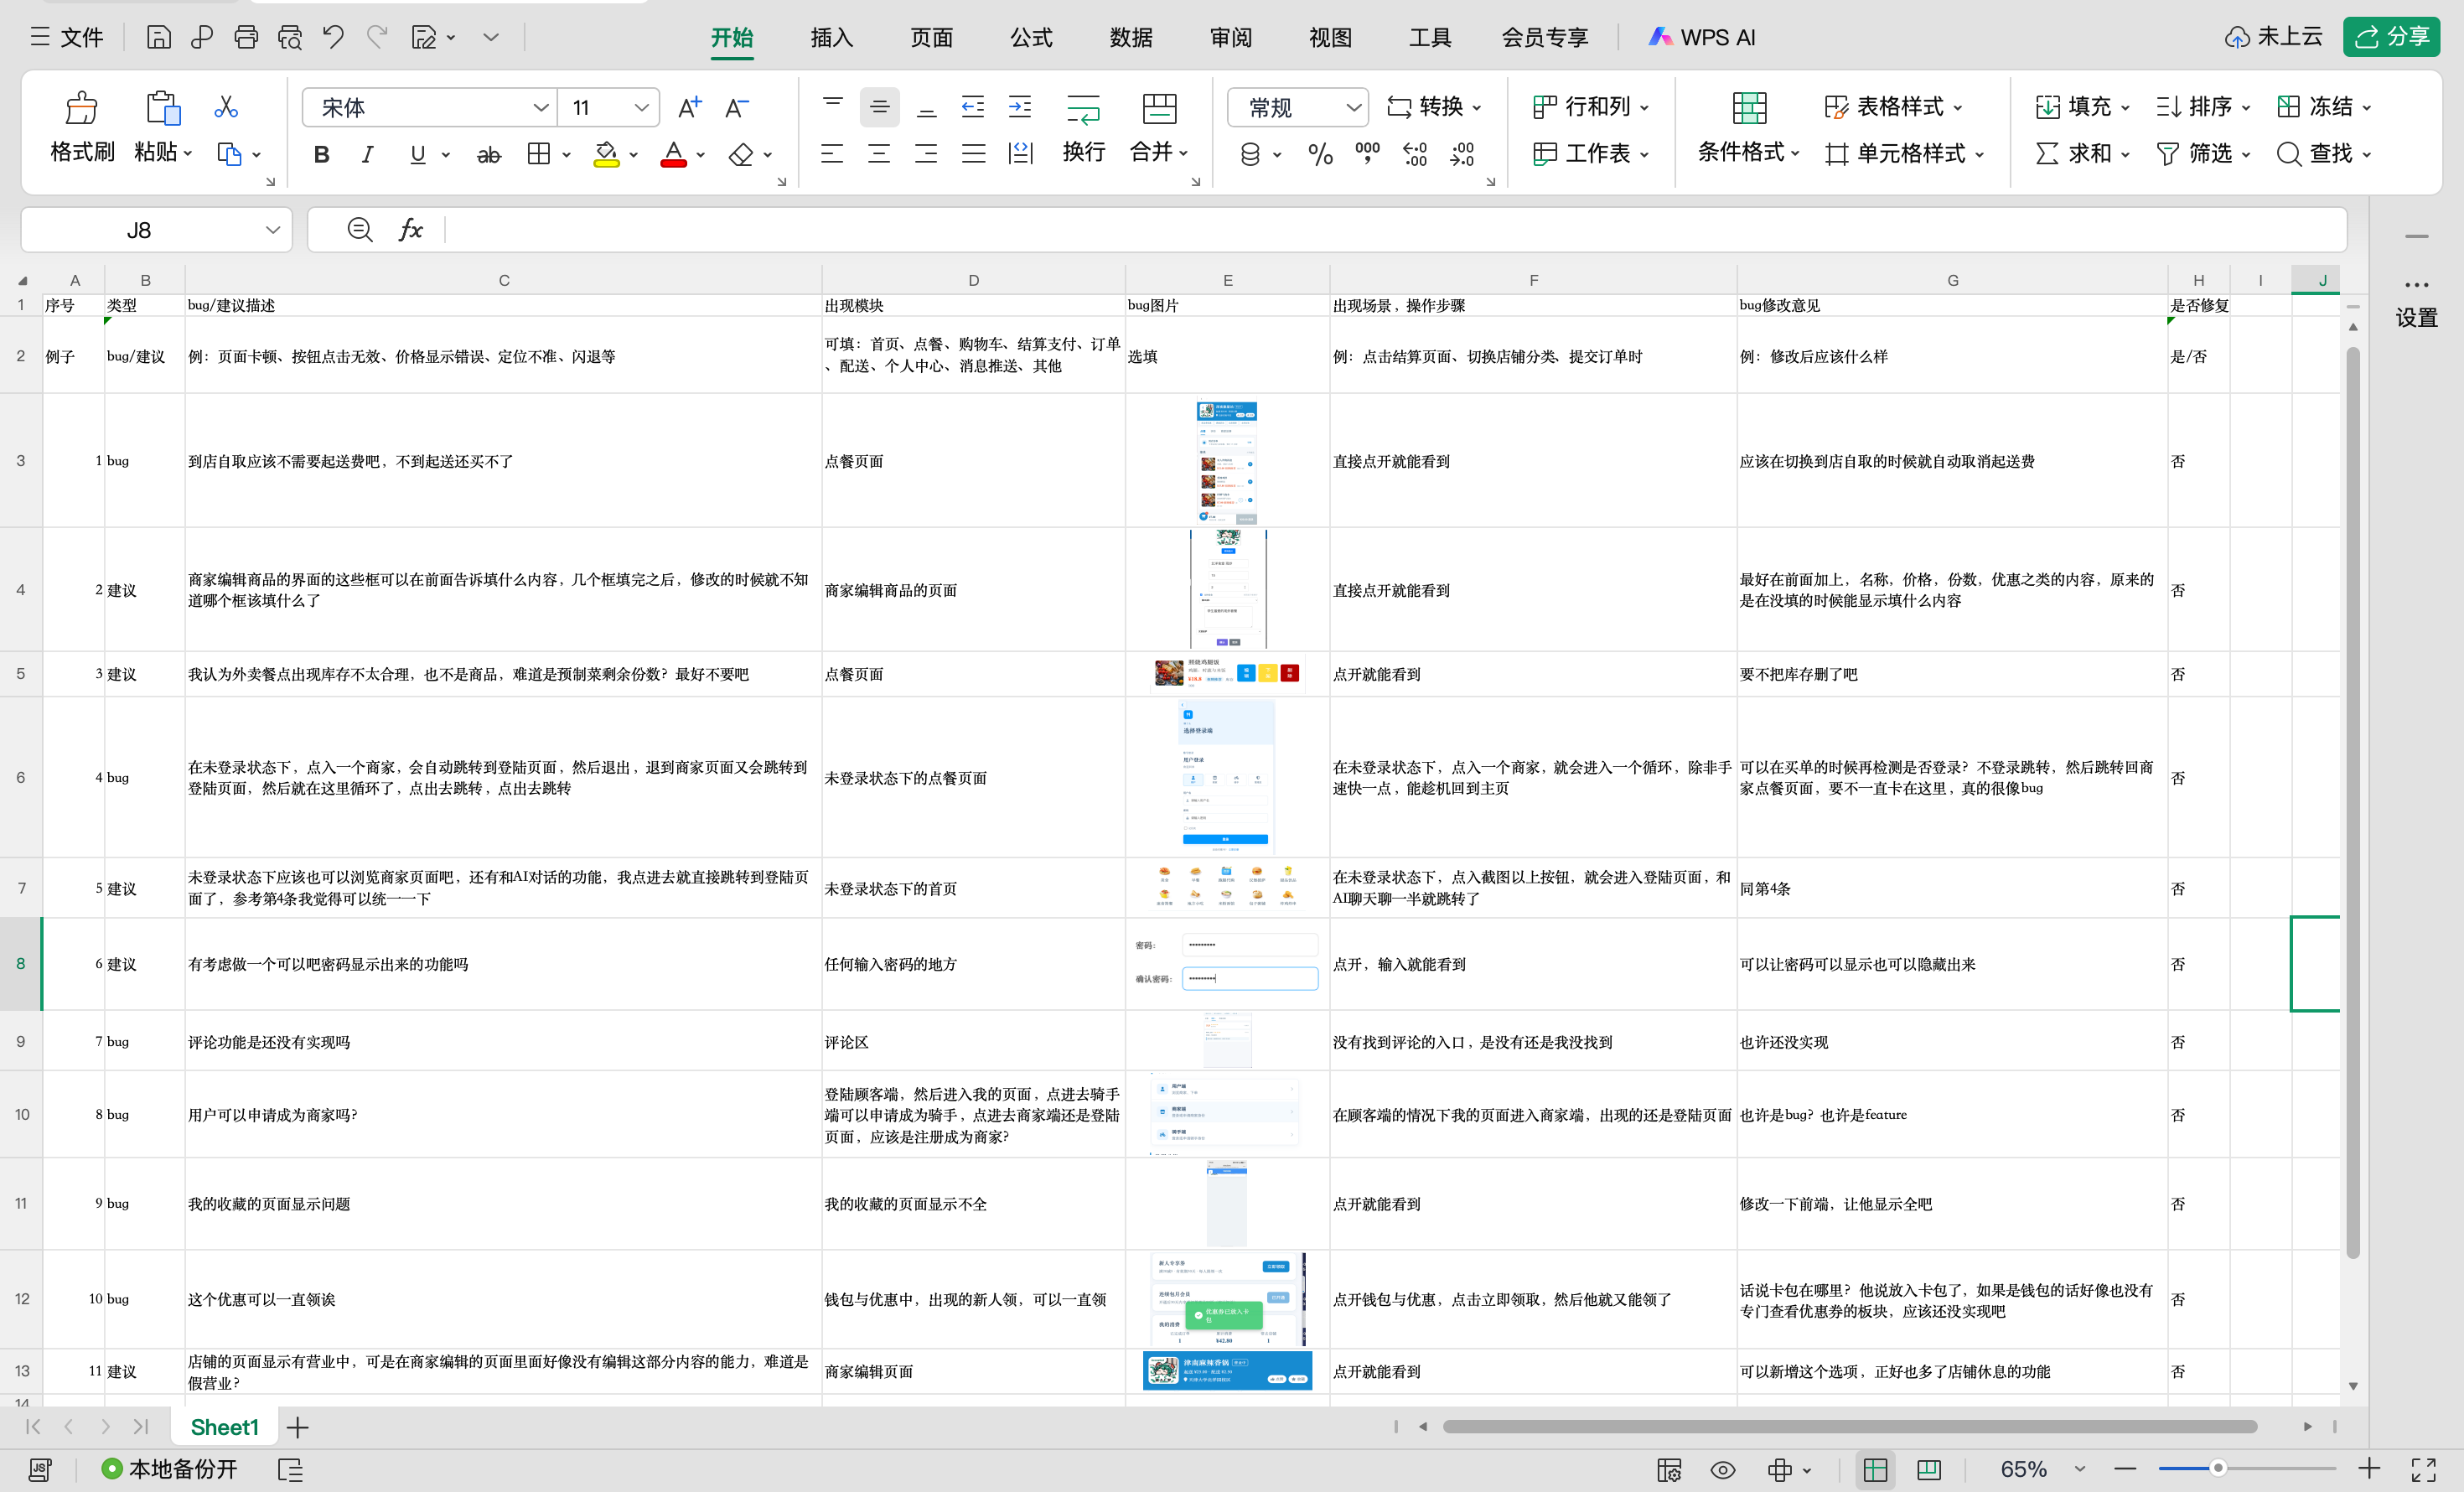
\includegraphics[width=.98\linewidth]{figures/report/process/bug-register.png}
  \caption{本组项目人工功能筛查使用的缺陷登记表（截图时状态）}
  \label{fig:process-bug-register}
\end{figure}

缺陷处理形成“发现问题—记录复现条件—确定责任模块—修改代码—重现原场景—检查关联业务—更新状态”的闭环。复测不仅检查原问题是否消失，还需要确认相关接口、页面和角色流程没有产生回归。人工筛查所得记录与自动化测试结果共同构成本组项目的内部测试证据；9月16日本组对其他小组开展的交叉验收另行记录，不与本表混用。
\section{界面测试}
界面测试以角色任务为单位进行。顾客需要完成查找、选购、确认费用与查看结果；商家需要能够快速识别待处理订单；骑手需要明确下一步动作；管理员需要看到审核依据和治理结果。统一风格只是基础，可理解的状态反馈和正确的操作约束更关键。
\begin{longtable}{L{.19\linewidth}L{.35\linewidth}L{.37\linewidth}}
\caption{界面验收检查清单（需结合浏览器执行）}\\\toprule 检查对象&操作场景&预期结果\\\midrule\endfirsthead\toprule 检查对象&操作场景&预期结果\\\midrule\endhead
登录与路由&未登录访问订单、登录后切换角色&引导到合法页面，不保留上一身份的私有内容。\\
列表与空状态&无店铺、无订单、接口延迟&展示空状态或加载反馈，不出现空白页。\\
购物车&增减数量、部分勾选、外送自取切换&数量、费用与地址要求一致，未提交商品保留。\\
支付&重复点击、失败、请求超时&按钮进入处理中，先确认权威结果，避免重复副作用。\\
骑手任务&任务被他人领取后再点击&明确提示并刷新任务，不显示虚假成功。\\
表单&必填缺失、格式错误、提交失败&指出具体字段，保留其他合法输入。\\
响应式&375 px 窄屏与桌面分辨率&关键内容与操作可见，横向溢出不遮挡按钮。\\
AI 入口&无凭证、超时、识别失败&解释原因并保留普通搜索与文本输入。\\\bottomrule
\end{longtable}
\section{单元测试与接口测试}
\subsection{后端规则测试}
仓库包含计价、资产、结算、推荐、通知和权限等测试。计价测试应覆盖普通用户与会员、起送价边界、满减、配送费和非法数量；资产测试应验证余额不足时不产生半完成扣减，取消后返还与原交易一致。

权限测试的重点是服务端信任边界。以 \code{OrderPricingTrustBoundaryTest} 为例，测试通过构造客户端参数与数据库价格不一致的情形，检查最终订单仍使用服务端数据。历史快照测试则验证商品名称改变后旧订单是否稳定。这些断言直接对应需求风险，比仅检查 HTTP 返回成功更有意义。
\subsection{前端测试的适用范围}
前端使用 Node 内置测试运行器，测试范围包括接口封装、路由、结算、支付视图、地址、主题和角色页面约束。部分测试检查源码结构和接口约定，部分调用真实工具函数或路由解析。这些测试适合发现低成本回归问题，但不等同于完整浏览器端到端测试。

因此，即便自动化套件全部通过，仍需执行浏览器中的加载、点击、表单、滚动和多角色会话验证。报告也不把浏览器开发者工具查看请求的人工调试称为严格意义上的单元测试。
\Needspace{8\baselineskip}
\subsection{典型测试文件与需求关联}
\begin{longtable}{L{.30\linewidth}L{.36\linewidth}L{.25\linewidth}}
\caption{代表性测试追踪关系}\\\toprule 需求关注点&仓库测试文件&主要验证内容\\\midrule\endfirsthead\toprule 需求关注点&仓库测试文件&主要验证内容\\\midrule\endhead
服务端权威计价&\code{OrderPricingTrustBoundaryTest.java}&不接受客户端伪造价格。\\
历史订单独立性&\code{OrderNameSnapshotJourneyTest.java}&订单名称快照的稳定性。\\
订单结算&\code{OrderSettlementServiceTest.java}&优惠、资产扣减与回退规则。\\
资料与地址归属&\code{ProfileAddressJourneyTest.java}&本人资料与地址操作边界。\\
配送状态&\code{DeliveryTaskStatusTest.java}&合法和非法状态转换。\\
AI 总体超时&\code{DeepSeekDeadlineTest.java}&重试不能无限延长总等待时间。\\
AI 会话授权&\code{AiChatHistoryMapperAuthorizationTest.java}&会话记录的访问边界。\\
前端结算与导航&\code{checkout.test.mjs}、\code{navigation.test.mjs}&结算逻辑和路由约束。\\\bottomrule
\end{longtable}
\section{四端联合测试}
联合测试按业务链路逐步扩展。先验证顾客下单与商家读取，再增加支付、出餐与骑手任务，最后加入确认收货、资产、评价和统计。某一步失败时，检查前一状态是否已经正确提交，避免把后续页面异常当作独立问题处理。
\begin{longtable}{L{.13\linewidth}L{.39\linewidth}L{.39\linewidth}}
\caption{端到端验收场景（需求清单，非通过记录）}\\\toprule 编号&执行步骤&核心断言\\\midrule\endfirsthead\toprule 编号&执行步骤&核心断言\\\midrule\endhead
E2E-01&顾客外送下单、模拟支付、商家接单出餐、骑手配送、顾客收货&四端状态可对应；订单、库存与资产不产生重复副作用。\\
E2E-02&顾客下单后修改商品名称价格，再查看原订单&原订单商品快照和交易金额不被当前配置改写。\\
E2E-03&顾客取消待支付或待商家处理订单，重复提交取消&取消规则生效，库存与资产仅恢复一次。\\
E2E-04&两名骑手同时领取同一任务&只绑定一人，另一人获得冲突反馈。\\
E2E-05&骑手上报异常，管理员处置后继续查询&任务与订单保持一致，处置记录可追踪。\\
E2E-06&用户描述预算与口味，查看候选并确认加入购物车&候选来自真实可售商品，确认前不改变购物车。\\
E2E-07&模拟外部 AI 超时，同时进行普通点餐&AI 按约定降级，核心交易仍可继续。\\
E2E-08&替换他人订单、地址、会话或任务编号&越权请求被拒绝，不返回私有数据。\\
E2E-09&创建自取订单并完成商家出餐与顾客取餐&不强制收货地址，不收外送费，不创建骑手任务。\\\bottomrule
\end{longtable}
\section{TDD 与需求变更测试}
课程要求通过“红—绿—重构”把需求落实为可执行约束。红阶段的失败应当来自缺少目标行为，而非依赖下载、端口占用或测试编译失败；绿阶段以最小必要实现满足断言；重构阶段再改善职责与结构，并保持原测试通过。

以历史价格问题为例，应先构造“下单后商家调价，原订单价格仍保持原值”的测试，再修改快照写入与查询；以骑手接单为例，应先表达任务已被领取时不能再次成功，再实现条件更新。这样的顺序使测试具有发现缺陷的能力，而不是实现完成后复制代码逻辑。

证明全程 TDD 需要提交历史、红阶段输出和对应改动共同支持。本次核对采用仓库当前快照，没有逐次审阅完整历史，因此不以测试文件数量推断整个开发过程均严格遵循 TDD。项目目录中的模拟练习材料也不作为真实开发历史或实测结果。
\section{本次复核结果及限制}
本次在代码快照 \code{17f80ab2} 中安装前端锁定依赖后，使用 Node.js 24.19.0 执行仓库既有前端测试：\textbf{235 项通过，0 项失败，0 项跳过}。执行日期为 2026 年 9 月 21 日，完整输出由项目组测试记录留存。仓库开发说明使用 Node.js 20，本次运行环境不同，应在正式验收时补充课程指定环境的复核。

同日使用 Eclipse Temurin JDK 21.0.6 运行后端 Maven Wrapper 测试（项目编译目标为 Java 17）：\textbf{340 项通过，0 项失败，0 项错误，0 项跳过}。测试类统计由当次 Surefire 报告汇总。本次模板重排未修改项目代码，也未重新执行业务测试。

性能压测、覆盖率报告、真实 AI 服务与浏览器全链路验收不包含在上述前端测试结果中。

\section{性能与 AI 并发验证方案}
SRS 的普通接口性能、20 并发抢单和核心服务覆盖率目标需要独立证据。压测应记录机器配置、数据库数据量、并发模型、请求分布、预热条件和持续时间，至少观察吞吐量、P50/P95/P99 延迟、错误率与数据库连接占用。

AI 场景应先使用可控的本地服务模拟延迟、429、5xx 和断连，再进行有限的真实服务验证。需要分别记录一次用户请求引起的首次模型调用数和重试次数，避免只统计成功答复而忽略失败成本。AI 压测同时运行普通订单查询，才能判断辅助功能是否挤占核心服务资源。

没有实际执行对应压测前，本报告不填写“支持多少并发”“响应时间降低多少”或“覆盖率达到多少”的数字。第五章中的容量计算属于解释风险的假设示例，不能作为验收结果。
